\section{Service guide}

The instructions below are meant to enable you to perform troubleshooting, repair and cleaning tasks adequately and without damaging the machine.

Read the respective guide carefully before you start to work on the HT500.3 3D Printer.


\subsection{Support requests - required information}

 In case you require support and contact us please always provide the following information:

\begin{itemize}
  \item Serial-no.
  \item Hardware revision
\end{itemize}

\begin{figure}[H]
  \centering
  \includegraphics[width=.7\linewidth]{./img/type_plate_ht500-3.png}
  \caption{Finding the hardware revision and serial-no. on the type plate.}
\end{figure}

\begin{itemize}
  \item The .log-file, downloaded via the web interface's Setup tab.
\end{itemize}

\begin{info}
  When downloading the .log-file via the web-interface, please open the \emph{Setup tab first} so that the currently set EEPROM data are written into the log.
  The log file saves all operating and communication commands since the initial commissioning and exports the last 20,000 commands into a data file. Due to this, it may require a few minutes for the system to gather all necessary data before the download menu appears. 
\end{info}

\begin{figure}[H]
  \centering
  \includegraphics[width=.7\linewidth]{./img/wi_v105-v110_logdownload.png}
  \caption{Downloading the log files via the web interface. Please remember opening the Setup tab first.}
\end{figure}

\begin{itemize}
  \item All system information provided on the \emph{Setup} menu. 
\end{itemize}

\begin{figure}[H]
  \centering
  \includegraphics[width=.7\linewidth]{./img/sg_setupmenu_information.png}
  \caption{Please send all system information of the GUI's Setup menu: software version, compatible hardware revision, microcontroller 
           firmware version (compatible and current).}
\end{figure}

Additionally, the following information may be helpful for examining and evaluating your specific request:

\begin{itemize}
  \item Photos of unsuccessful prints often give a clue of what may have gone wrong.
  \item G-codes of above mentioned prints \emph{and} the respective .stl-data allow for reprinting and reproducing your print job and help 
        identifying faults.
  \item Photos and short videos of components, be they damaged or behaving oddly, always provide some clarification.
\end{itemize}



\subsection{Packing and transport safeguarding}

If the HT500.3 is to be shipped (e.g. for a full manufacturer's in-house inspection), it must be thoroughly packed and all moving components must be carefully secured against shifting to avoid transportation damages. 

\begin{info}
   Replacement of parts damaged due to improper transport securing will be carried out at \emph{your costs}. 
\end{info}


\subsubsection{Safeguarding of movable components}

 You will need the following material:

\begin{itemize}
  \item removable strapping tape
        (e.g. tesa® Strapping 64250, Scotch® Strapping Tape 8898 Blue)
  \item packing foam foil
        (any PE-foam for common packing applications)
  \item cardboard
\end{itemize}

The following description assumes that:

\begin{itemize}
  \item all axes are in their respective home position;
  \item filament has been unloaded and the 3D Printer has at least been briefly cleaned;
  \item the 3D Printer has been switched off, disconnected from the power supply and cooled down;
  \item all cables have been removed from the rear side.
\end{itemize}



The first and most important component to be secured is the extruder head. It is \emph{mandatory} to fix it exactly as shown here. Otherwise sensors and other components may be damaged beyond repair and must be replaced.

\begin{itemize}
  \item Move the H-gantry to the front and the extruder head to the right-hand side.
  \item Place a foam coil between the extruder head and the right X-axis shaft carriage and push the extruder head against the coil.
  \item Fasten the extruder head together with the carriage by entwining them with strapping tape.
  \item Make sure to tension the tape so that any extruder head movement is prevented.
\end{itemize}

 

\begin{figure}[H]
  \centering
  \includegraphics[width=.7\linewidth]{./img/packstep0.png}
  \caption{Move the extruder head to the front and to the right.}
\end{figure}

\begin{figure}[H]
  \centering
  \includegraphics[width=.7\linewidth]{./img/secure_extruderhead.png}
  \caption{Cushion the extruder head with the foam coil against the right carriage and tightly fasten it with tape.}
\end{figure}

\begin{itemize}
  \item Fasten the energy chain to the printer top cover. 
\end{itemize}

\begin{figure}[H]
  \centering
  \includegraphics[width=.7\linewidth]{./img/secure_echain.png}
  \caption{Entwine the e-chain with tape and fasten it to the printer's top cover.} 
\end{figure}

\begin{itemize}
  \item Fix the H-gantry with strapping tape against forward movement by fastening it to one of the Z-Axes. 
\end{itemize}

\begin{figure}[H]
  \centering
  \includegraphics[width=.7\linewidth]{./img/secure_hbridge_rear.png}
  \caption{Entwine the hind shaft of the H-gantry with tape and fasten it to on of the Z-axes.}
\end{figure}

\begin{itemize}
  \item Fix the H-gantry with strapping tape against backward movement by fastening it to the printer top cover.
  \item Make sure to tension the tape to prevent forward/backward movement of the H-bridge. 
\end{itemize}

\begin{figure}[H]
  \centering
  \includegraphics[width=.7\linewidth]{./img/secure_hbridge_front.png}
  \caption{Entwine the frontal shaft of the H-bridge with tape and fasten it to the printer's top cover.}
\end{figure}

\begin{itemize}
  \item Cut and prepare a cardboard support as depicted.
  \item Place the support underneath the print table and fix it with strapping tape.
\end{itemize}

\begin{figure}[H]
  \centering
  \includegraphics[width=.7\linewidth]{./img/img_1708.jpg}
  \caption{The cardboard support installed at delivery is the best option to secure the print table.}
\end{figure}

\begin{figure}[H]
  \centering
  \includegraphics[width=.7\linewidth]{./img/secure_printtable.png}
  \caption{Place the cardboard support underneath the print table and fix it with tape.}
\end{figure}

\begin{itemize}
  \item Close the build chamber doors and fix them with strapping tape as shown.
  \item Wrap the touchscreen with foam foil and fixate it with strapping tape.
\end{itemize}


\begin{figure}[H]
  \centering
  \includegraphics[width=.7\linewidth]{./img/secure_doors_gui.png}
  \caption{Tape the doors and wrap the touchscreen with foam foil.}
\end{figure}


\subsubsection{Packing for transport}

After safeguarding, the 3D Printer is ready for packing. You will need the following material:

\begin{itemize}
  \item 4x lashing strap or tension belt
  \item closed surface transport pallet
  \item packing foam foil
  \item 4x anti-slip mats 50 x 50 mm (only 3D Printers without rubber feet)
  \item OSB transport top cover (or similar) 700 x 700 x 25 mm
  \item delivery transport box side cover frame
  \item delivery transport box lid
\end{itemize}

The description refers to using the original transport box the 3D Printer was delivered in. If you disposed of the box, make sure to provide adequate replacement.

\begin{itemize}
  \item Lift the 3D Printer onto the center of the pallet.
  \item Place a suitable piece of transport foam foil on top of the 3D Printer.
\end{itemize}

\begin{notice}
  To avoid damage by slipping, place anti-slip mats under the feet if your 3D Printer is not already equipped with rubber feet.
  \begin{figure}[H]
    \centering
    \includegraphics[width=.7\linewidth]{./img/packstep3.png}
  \end{figure}
\end{notice}

\begin{figure}[H]
  \centering
  \includegraphics[width=.7\linewidth]{./img/packstep1.png}
  \caption{Place the 3D Printer in the middle of the pallet and cover it with foam foil.}
\end{figure}

\begin{itemize}
  \item Place the cover plate on top of the 3D Printer. 
\end{itemize}

\begin{figure}[H]
  \centering
  \includegraphics[width=.7\linewidth]{./img/packstep4.png}
  \caption{The cover plate protects the printer when strapping it down.}
\end{figure}

\begin{itemize}
  \item Fasten the 3D Printer with two lashing straps to the pallet.
\end{itemize}

\begin{figure}[H]
  \centering
  \includegraphics[width=.7\linewidth]{./img/packstep5.png}
  \caption{The 3D Printer must be tightly secured on the transport pallet.}
\end{figure}

\begin{itemize}
  \item Lift the side cover frame onto the pallet.
  \item Make sure that the grove of the pallet fits smoothly.
\end{itemize}

\begin{figure}[H]
  \centering
  \includegraphics[width=.7\linewidth]{./img/packstep6.png}
  \caption{The side cover frame must be accurately positioned to protect the 3D Printer from damage.}
\end{figure}

\begin{itemize}
  \item Close the box with the lid.
  \item Make sure that the lid smoothly fits into the side cover frame. 
\end{itemize}

\begin{figure}[H]
  \centering
  \includegraphics[width=.7\linewidth]{./img/packstep7.png}
  \caption{Ensure the lid fits so that tensioning the lashing straps will work.}
\end{figure}

\begin{itemize}
  \item Secure the transport box with two lashing straps on the pallet.
  \item Attach all necessary labeling on the outside:
    \begin{itemize}
      \item dispatch note
      \item UP sticker (present on the original transport box)
      \item FRAGILE sticker (present on the original transport box)
      \item PROTECT FROM WEATHER EFFECTS (if required, present on the original transport box)
    \end{itemize}
\end{itemize}

\begin{figure}[H]
  \centering
  \includegraphics[width=.7\linewidth]{./img/packstep8.png}
  \caption{The HT500.3 3D Printer is packed and ready for transportation 
           after lashing straps have been tightened and all labeling has been attached.}
\end{figure}



\subsection{Hardware components and manual tasks}


\subsubsection{Maintenance Intervals}

\paragraph{Daily (end of shift)}

\begin{table}[H]
  \centering
  \begin{tabulary}{\textwidth}{ L L L }
    \toprule
    Where          &	    What                      &	 	Tools / To Do \\
    \midrule
    Build chamber  &	 	remove filament residues  &	 	brush, hand broom, vacuum cleaner \\
    \bottomrule
  \end{tabulary}
\end{table}    

\paragraph{Monthly (150 operating hours)}  

\begin{table}[H]
  \centering
  \begin{tabulary}{\textwidth}{ L L L }
    \toprule
    Where               &	  What                                                     &	 Tools / To Do \\
    \midrule
    Timing belt         &	  check the tension; re-tension if required                &	 $\rightarrow$ section \ref{sec:belttension} \\
    Shafts              &	  check for dryness; lubricate if required                 &	 $\rightarrow$ section \ref{sec:lubrication} \\
    Cooling circuit     &	  check hoses for excessive bubbles; refill if required    &   $\rightarrow$ section \ref{sec:coolant} \\
                        &	  check hose connectors at the LEDs and 
                              the stepper drives for correct positioning; 
                              refasten if required 	                                   &                  \\
    Dust wiping sponge  &	  check for cleanliness; 
                              clean or replace if required                             &  rinse with fresh water
                                                                                          and dry thoroughly \\
    \bottomrule
  \end{tabulary}
\end{table}


\paragraph{Yearly (2.500 operating hours)}

\begin{table}[H]
  \centering
  \begin{tabulary}{\textwidth}{ L L L }
    \toprule
    Where             &     	  What                                                   &	 Tools / To Do \\
    \midrule
    Z-axis 
    spindle drive 	  &  check for fast seat:\newline
                         with the 3D Printer switched on, grab the print table near
                         the elevator and try to lift it\newline
                         $\rightarrow$ play of the table on  the spindle requires 
                         replacement of the spindle nut\newline                                  
                         $\rightarrow$ if you can lift the entire assembly including 
                         the spindle, the adjusting rings must be refastened 	         &   $\rightarrow$ section \ref{sec_spindlecollar}  \\
    \bottomrule
  \end{tabulary}
\end{table}

\subsubsection{Cleaning recommendation}

\begin{danger}
   OF INJURY\\
   Some plastics need very aggressive solvents that may cause intoxication, caustic burns, skin, eye and/or mucosal irritations, allergic reactions and other medical consequences. Solvents may emit flammable or toxic vapors or be corrosive.
   To avoid injuries and accidents due to use of solvents:

   \begin{itemize}
      \item Always observe the safety information provided in the manufacturer's safety data sheet concerning
            possible dangers, handling and adequate storage.
      \item Always wear adequate protective equipment.
      \item Do not use solvents in a surrounding not suited to the task. If required, 
            adequate aeration or exhaust ventilation has to be provided.
      \item Always use adequate containers for handling and storing solvents.
      \item It is the owner's responsibility to provide any necessary equipment and protective gear 
            for every person operating the HT500.3 3D Printer.
  \end{itemize}
\end{danger}

\begin{danger}
  OF BURNING\\
  The build chamber interior may reach temperatures of up to 70\degree C (158\degree F), the print bed may reach temperatures up to 130\degree C (266\degree F) and 
  the hot ends may reach temperatures up to 300\degree C (572\degree F). Touching components can cause burning injuries ranging from burn blisters to medium aching burns. Before cleaning any component inside the build chamber:
  
  \begin{itemize}
    \item Move the print head to the maintenance position 
          (GUI $\rightarrow$ \lbrack Expert Control\rbrack  $\rightarrow$ \lbrack Print Head Maintenance Position \rbrack  ).
    \item Switch preheating of the 3D Printer off 
          (GUI $\rightarrow$ \lbrack Print\rbrack  $\rightarrow$ \lbrack Preheat Chamber/Bed OFF\rbrack  ).
    \item Let the printer cool down to at least 52\degree C.
  \end{itemize}
\end{danger}

\begin{notice}  
  Acetone is the most effective solvent for ABS and thus recommended for most cleaning purposes at the HT500.3 3D Printer.
  To remove residues of other plastics than ABS, refer to the respective manufacturer's data sheet for suitable solvents.

  Regard the following when using solvents for cleaning purposes:

  \begin{itemize}
    \item Do not use solvents inside the build chamber. They may evaporate and produce fumes that can dissolve plastic 
          components (e.g. the energy chain links) and printed objects. Always remove components from the build chamber before treating them with a solvent and dry thoroughly before re-insertion.
    \item Do not use liquids inside the build chamber. These may enter the electronic chamber and cause short circuits or
          otherwise damage electronic components.
  \end{itemize}
\end{notice}


\paragraph{Housing}

Although during normal operation it is not necessary to clean the 3D Printer daily, regularly dusting reduces the probability of dust entering the feed system and causing clogging. Also, the visual appearance of the 3D Printer is improved and damaged components are more easily detected.
All components of the HT500.3s' housing can be cleaned with mild household detergents (e.g. dish soap, glass cleaner) and lint-free towels.
\emph{Do not} use abrasive detergents or scouring pads as these will scratch and blind the acrylic glass covers and the touchscreen surface.
Material residues should be removed routinely from the build chamber. Use a soft brush or a low-running vacuum cleaner to remove loose material shreds.

\paragraph{Touchscreen}

If required, use a microfiber or spectacle cloth moistened with glass cleaner to wipe the touchscreen.

\paragraph{Print bed}

PEI is highly resistant to a lot of solvents. It is particular compatible with acetone and isopropyl alcohol. If you experience insufficient adhesion of objects to the surface during prints, it is advisable to thoroughly clean the print bed with an acetone-soaked lint-free cloth.

Grease residues on the surface of the print bed (i.e. fingerprints) can lead to poor adhesion. To degrease, apply isopropylalcohol to a lint-free cloth and thoroughly wipe the surface. During further use, regular removal of grease residues with isopropyl alcohol will prevent poor adhesion.

Use acetone as solvent to remove ABS residues from the print bed. Apply the acetone to a cloth and wipe the print bed rather than dousing it directly.

Other material's residues are best removed with a lint-free towel soaked in a suitable, non-corrosive, non-toxic solvent. Observe the manufacturer's safety data sheet when handling plastic solvents. Make sure to thoroughly wash off any residues. Remaining smear may lead to increased adhesion, which can render it impossible to release printed objects without damage.

\paragraph{Hot ends}

Cleaning the hot end nozzle tip is required quite often compared to other components of the 3D Printer. Dust ingression through the filament supply system, coking of material, and storage in a dusty place may lead to clogging of the tip's bore.
An imprecisely (too closely) leveled print bed, too low extrusion temperatures or too high an extrusion speed can lead to the nozzle tip choking itself.
In any of these cases, a decreasing print quality and slipping of the drive gear will be the first visible effects. Removing and cleaning the nozzle tip is then necessary; the description below should remedy the problem, as long as no hardware defect is present.

Cleaning the extruder nozzle is only required if it is clogged with coked material or foreign particles. It is recommended after dissembling the hot end at material change (installing a \emph{different} material). 

\begin{info}
  In areas with high dust formation, \underline{especially} from textile fibers and similarly flexible particles, the risk of the nozzles to become clogged is highly increased.
\end{info}

\paragraph{Filament drive gear}

Slipping of the drive gear is almost always the first and visible consequence of a clogged nozzle.
Other conditions (e.g. too high idler tension) may also cause the drive gear to grind into the filament and fill with abrasion. Material transport will stop and the print job will not be finished.
Regard that the printer will nevertheless continue to print if not aborted by the operator.
Clean according to the description below

\begin{figure}[H]
  \centering
  \includegraphics[width=.7\linewidth]{./img/mtc_cleangeardrive.png}
  \caption{Filament abrasion at the drive gear due to slipping.}
\end{figure}

\subsubsection{Changing the filament} \label{sec:filamentchange}

When the filament limit switch at the filament supply registers the end of the filament strand on the spool, the 3D Printer stops automatically and signals lack of material at the touchscreen.
If you want to remove the filament for other reasons (e.g. to use a differently colored material), the following description applies also.


\paragraph{Required tools}

\begin{itemize}
  \item diagonal cutters
\end{itemize}


\paragraph{Unloading Filament}


\begin{enumerate}
  \item Go to the \emph{[Expert Control]} menu and heat up your extruder to melting temperature.
  \item Pull the filament feeding tube out of the extruder idler lever about 3cm.
  \item Cut the filament with wire cutters about 1cm above the extruder idler lever.
  \item Cut the filament with wire cutters between filament feed insert and
        filament spool at the back of the machine.
  \item From inside of the build chamber, pull the separated strand of filament out of 
        the feeding tube.
  \item Pivot the filament idler wheel away from the filament drive gear with two fingers,
        and pull the remaining filament section upwards out of the nozzle.
  \item In the \emph{[Expert Control]} panel, switch your extruder heater OFF again.
\end{enumerate}


\paragraph{Loading Filament}

If you want to continue printing with another type of plastic (e.g. PETG instead of ABS) than has previously been used in the currently installed nozzle, you need to change the extruder nozzle before loading the filament.

\begin{info}
  Using the same extruder nozzle for materials with different properties may lead to clogging of the nozzle tip due to coking or sooting.
  Kühling\&Kühling recommend either thorough cleaning of the extruder nozzle with a suitable solvent and pipe cleaners or using a single nozzle for every type of material.
\end{info}

\begin{enumerate}
  \item Unload the current filament as described in the previous paragraph.
  \item Subsequent to unloading you have to change the extruder nozzle as 
        described in the Service guide.
  \item Install a new spool of filament by sliding it onto the spool holder at the back of
        the machine. Adjust the spool carrier to fit.
  \item Pull the filament feed tube out of the extruder idler lever.
  \item Cut off the beginning of the filament with wire cutters to get a
        straight end.
  \item Lead the plastic rod into the filament feed until it protrudes the feeding tube
        about 10cm at the other side (at the extruder).
  \item Relax the filament idler wheel tension with two fingers.
        Then feed the filament from top through the idler lever,
        down into the nozzle.
  \item Go to the \emph{[Expert Control]} menu and heat up your extruder to melting temperature.
  \item Use the \emph{extrude} controls to manually prime the nozzle until a consistent, smooth strand of extruded material
        flows out of the nozzle tip.
  \item In the \emph{[Expert Control]} panel, switch your extruder heater OFF again.
\end{enumerate}

\begin{info}
  Make sure to choose the appropriate filament profile from the material database.
\end{info}


\subsubsection{Adjusting the spool carriers}

\paragraph{Required tools}
 
\begin{itemize}
  \item Allen wrench \#2.5
\end{itemize}

\paragraph{Procedure}

If you want to use a different filament spool diameter (less or more material), you have to adjust the spool carrier position.

\begin{info}
  With an appropriate Allen key you can carry out the following steps without removing the filament spool.
\end{info}
\begin{itemize}
  \item Use the Allen key to loosen the fixing screws of the carrier.

  \begin{figure}[H]
    \centering
    \includegraphics[width=.7\linewidth]{./img/mtc_filamentmovespools.png}
    \caption{Loosening the fixing screws of spool carriers.}
  \end{figure}

  \item Slide the carrier to or away from the filament inlet to a position that 
        leaves approximately 1 cm between the spool's outer rim and the limit switch. Make sure that the filament enters the inlet at an angle 
        of 85-90\degree.
  \item Refasten the fixing screws.

  \begin{figure}[H]
    \centering
    \includegraphics[width=.7\linewidth]{./img/mtc_filamentinletmeasures.png}
    \caption{Admissible distance and inlet angle.}
  \end{figure}

\end{itemize}


\subsubsection{Remedying clogging}

\paragraph{Required tools}

\begin{itemize}
  \item dental pick hook or needle
  \item material specific solvent
  \item pipe cleaner
\end{itemize}

\paragraph{Procedure}

\begin{itemize}  
  \item Unload the filament ($\rightarrow$ section \ref{sec:filamentchange}).
  \item Screw off the nozzle.
  \item Roughly remove material residues mechanically (e.g. using a brass wire brush - wear protective goggles!).
  \item Drop the nozzle tip into a suitable solvent and wait for the residues to be loosened or completely dissolved.
  \item Remove remaining material mechanically.
  \item Dry the nozzle thoroughly before re-installation.
\end{itemize}

To remove particles and abrasion from the feed system:

\begin{itemize} 
  \item Remove the filament strand from the supply system.
  \item Take out the dust wiping sponge from the filament inlet, rinse it with water, and dry it thoroughly.
  \item  Scrape the teeth of the drive gears with a pointed tool (e.g. dental pick).
  \item  Reinstall the supply hoses and the dust wiping sponge.
\end{itemize}

\paragraph{Completion}

After having re-installed or exchanged all components, 
reload the filament, prime the extruders and run the \lbrack Print bed leveling\rbrack  wizard. 


\subsubsection{Shaft lubrication} \label{sec:lubrication}

All linear bearings of the HT500.3 are equipped with linear ball bearings. The shafts may accumulate dirt or condensation. Slightly Lubricating/Cleaning the shafts may then be necessary.

\paragraph{Required tools}

\begin{itemize}
  \item \emph{HIWIN Type G05} bearing grease
  \item paper towel or lint-free cloth
\end{itemize}

\begin{notice}
  Do not use any other lubricant. The linear bearings may get irreparably damaged when greased falsely. 
\end{notice}

\paragraph{Applying lubricant}

If you notice strong vibrations of the print table during homing and leveling or if your printed objects show increasingly rough vertical irregularities:

\begin{itemize}
  \item Wipe shafts clean with a paper towel.
  \item Coat the shafts with a thin layer of the lubricant.
\end{itemize}

\subsubsection{Opening the electronic chamber}

To access the cooling system or the control elements, you have to remove the left or the right side cover panel. The description below applies to either side. 

\begin{danger}
  ELECTRIC SHOCK HAZARD\\
  Electric shock can cause severe injuries. Never open the electronic chamber when the 3D Printer is powered on.
  Always shut down and power off the 3D Printer and disconnect the power supply before removing covers and working on electronic components. Allow the power supply to discharge for at least one minute. 
\end{danger}

\begin{notice}
  Electrostatic discharge can damage electronic components. Ground yourself before touching electronics. 
\end{notice}

\paragraph{Required tools}
\begin{itemize}
  \item Allen wrench \#2.5 
\end{itemize}

\paragraph{Additional information}

Software manual

\paragraph{Removing}

Shut down the printer via the touchscreen panel, switch off the main power switch and unplug the supply cable. Open the electronic chamber of the 3D Printer in the following sequence:

\begin{itemize}
  \item Slightly tilt the apparatus to the opposing side and place a square length of wood underneath the bottom.
\end{itemize}

\begin{danger}
  OF CRUSHING\\
  Capsizing of the 3D Printer can cause crushing injuries and damage the housing beyond repair. Make sure the apparatus does not topple. 
\end{danger}

\begin{itemize}
  \item Loosen (\emph{do not remove}) the hexagon socket screws of the feet and the upper hind cover angle.
  \item Turn the hammerhead nuts by 90\degree.
  \item Remove the feet and the angle.
  \item Loosen (\emph{do not remove}) the hexagon socket screws of the cover panel.
  \item Turn the hammerhead nuts by 90\degree.
  \item Remove the cover panel.
  \item Loosen all screws around the white acrylic side panel and take the panel off. 
        You now have access to the electronics driving the HT500.3.
\end{itemize}

Reinstall in reverse order, remove the wood and restart.

\begin{figure}[H]
  \centering
  \includegraphics[width=.7\linewidth]{./img/sg_openechamber_1.png}
  \caption{Lift the 3D Printer at one side; the feet and the hind cover angle must be removed.}
\end{figure}

\begin{info}
  You want to keep the t-slot nuts on the thread – otherwise they might fall into the slot, which can require further disassembling of the printer to get it back out.
\end{info}

\begin{figure}[H]
  \centering
  \includegraphics[width=.7\linewidth]{./img/open_electronics_enclosure_-_step4_-_02.png}
\end{figure}

\begin{figure}[H]
  \centering
  \includegraphics[width=.7\linewidth]{./img/open_electronics_enclosure_-_step4_-_03.png}
\end{figure}

\begin{figure}[H]
  \centering
  \includegraphics[width=.7\linewidth]{./img/open_electronics_enclosure_-_step4_-_04.png}
\end{figure}

\begin{figure}[H]
  \centering
  \includegraphics[width=.7\linewidth]{./img/open_electronics_enclosure_-_step5_-_02.png}
\end{figure}

\begin{figure}[H]
  \centering
  \includegraphics[width=.7\linewidth]{./img/open_electronics_enclosure_-_step5_-_03.png}
\end{figure}

\begin{figure}[H]
  \centering
  \includegraphics[width=.7\linewidth]{./img/open_electronics_enclosure_-_step5_-_01.png}
\end{figure}

\subsubsection{Changing the nozzle tip}

Printing with another nozzle diameter, cleaning or change of material all requires unscrewing and remounting the nozzle tip. Although not a complicated procedure, make sure to read the following description thoroughly to avoid damaging the hot-end. 

\begin{danger}
  BURNING HAZARD\\
  Before unscrewing a nozzle, the filament must be removed from the hot-end which may require heating to extrusion temperature. Depending on the installed material temperatures up to 300\degree C may be necessary that can cause severe burns.

  \begin{itemize}
    \item Be careful not to touch hot components.
  \end{itemize}
\end{danger}

\paragraph{Required tools}

\begin{itemize}
  \item open-jaw wrench size 4
\end{itemize}

\paragraph{Removing the nozzle}

After the extruder has cooled down:

\begin{itemize}
  \item Open the <Expert Control> menu, tap the \lbrack Printhead Maintenance Position\rbrack  button 
        and wait until the print head has moved to the middle front position.
  \item Check nozzle adapter thumb screw for tightness.
\end{itemize}


\begin{notice}
  If solidified material hinders loosening the nozzle effortlessly, heat up the extruder to the specific extrusion temperature and loosen the tip 2 or 3 turns. Do not unscrew the heated nozzle totally. Dropping the hot nozzle will damage the acrylic bottom. Afterwards, turn the extruder off and wait until it has cooled down before completely removing the nozzle. 
\end{notice}

\begin{itemize}
  \item Loosen and remove the nozzle with a size 4 wrench at the width flat of the nozzle. Carefully slide the nozzle out of
        the heating element.
\end{itemize} 

\paragraph{Installing a new nozzle}

\begin{itemize}
  \item Slide a new nozzle into the heating element.
  \item Screw the nozzle into the nozzle adapter. 
  \item Carefully fasten the nozzle with a size 4 wrench.
  \item Run the Print Bed Leveling wizard. 
\end{itemize} 


\subsubsection{Refilling the cooling circuit} \label{sec:coolant}

Thermal cycles and diffusion of the coolant makes refilling the cooling circuit necessary approximately every four weeks. To refill the coolant circuit, follow the instructions given below. 

\paragraph{Required tools}

\begin{itemize}
  \item Coolant Innovatek Protect IP ready-to-use \footnote{Order directly via sales@kuehlingkuehling.de, 
        the manufacturer's webshop (http://innovatek.de, manufacturer part number: 500473) or related distributors.} 
        (max. 250 ml)
  \item Allen wrench \#2.5
\end{itemize}

\paragraph{Checking the cooling circuit}

\begin{info}
  Lack of coolant may lead to damage of the affected components, especially the LEDs. Too much air in the cooling circuit leads to clogging of the copper connectors due to oxidation.
  Check the cooling circuit regularly for excess amounts of gas bubbles.
\end{info}

The amount of gas bubbles in the cooling circuit is the indicator for refilling. A small amount of bubbles always circles the hoses and can be considered normal. To asses whether the cooling circuit must be refilled, check the following:

\begin{itemize}
  \item The bubbles are small and running freely $\rightarrow$ there is no need for refilling the cooling circuit.
  \item Bubbles reach the size of the hose's diameter, are sticking in places and do not disappear 
        a few minutes after switching the build chamber on $\rightarrow$ refill as described below.
\end{itemize}

\paragraph{Refilling the pump}

\begin{enumerate}
  \item Locate the water pump at the rear of the machine.
  \item Remove the pump's lid by turning it counterclockwise and pulling it off.
  \item Refill with coolant up to the level indication.
  \item Let the pump run for some minutes. Monitor the coolant hoses and check that air bubbles run freely.
        If necessary, carefully flick the hoses to free trapped air. When all air bubbles have left the cooling system, check the filling level of the pump again and refill to the upper limit.
  \item Press the lid into the housing and turn it clockwise. Make sure the lid is positioned fast 
        in its seat and locked.
\end{enumerate}

\begin{figure}[H]
  \centering
  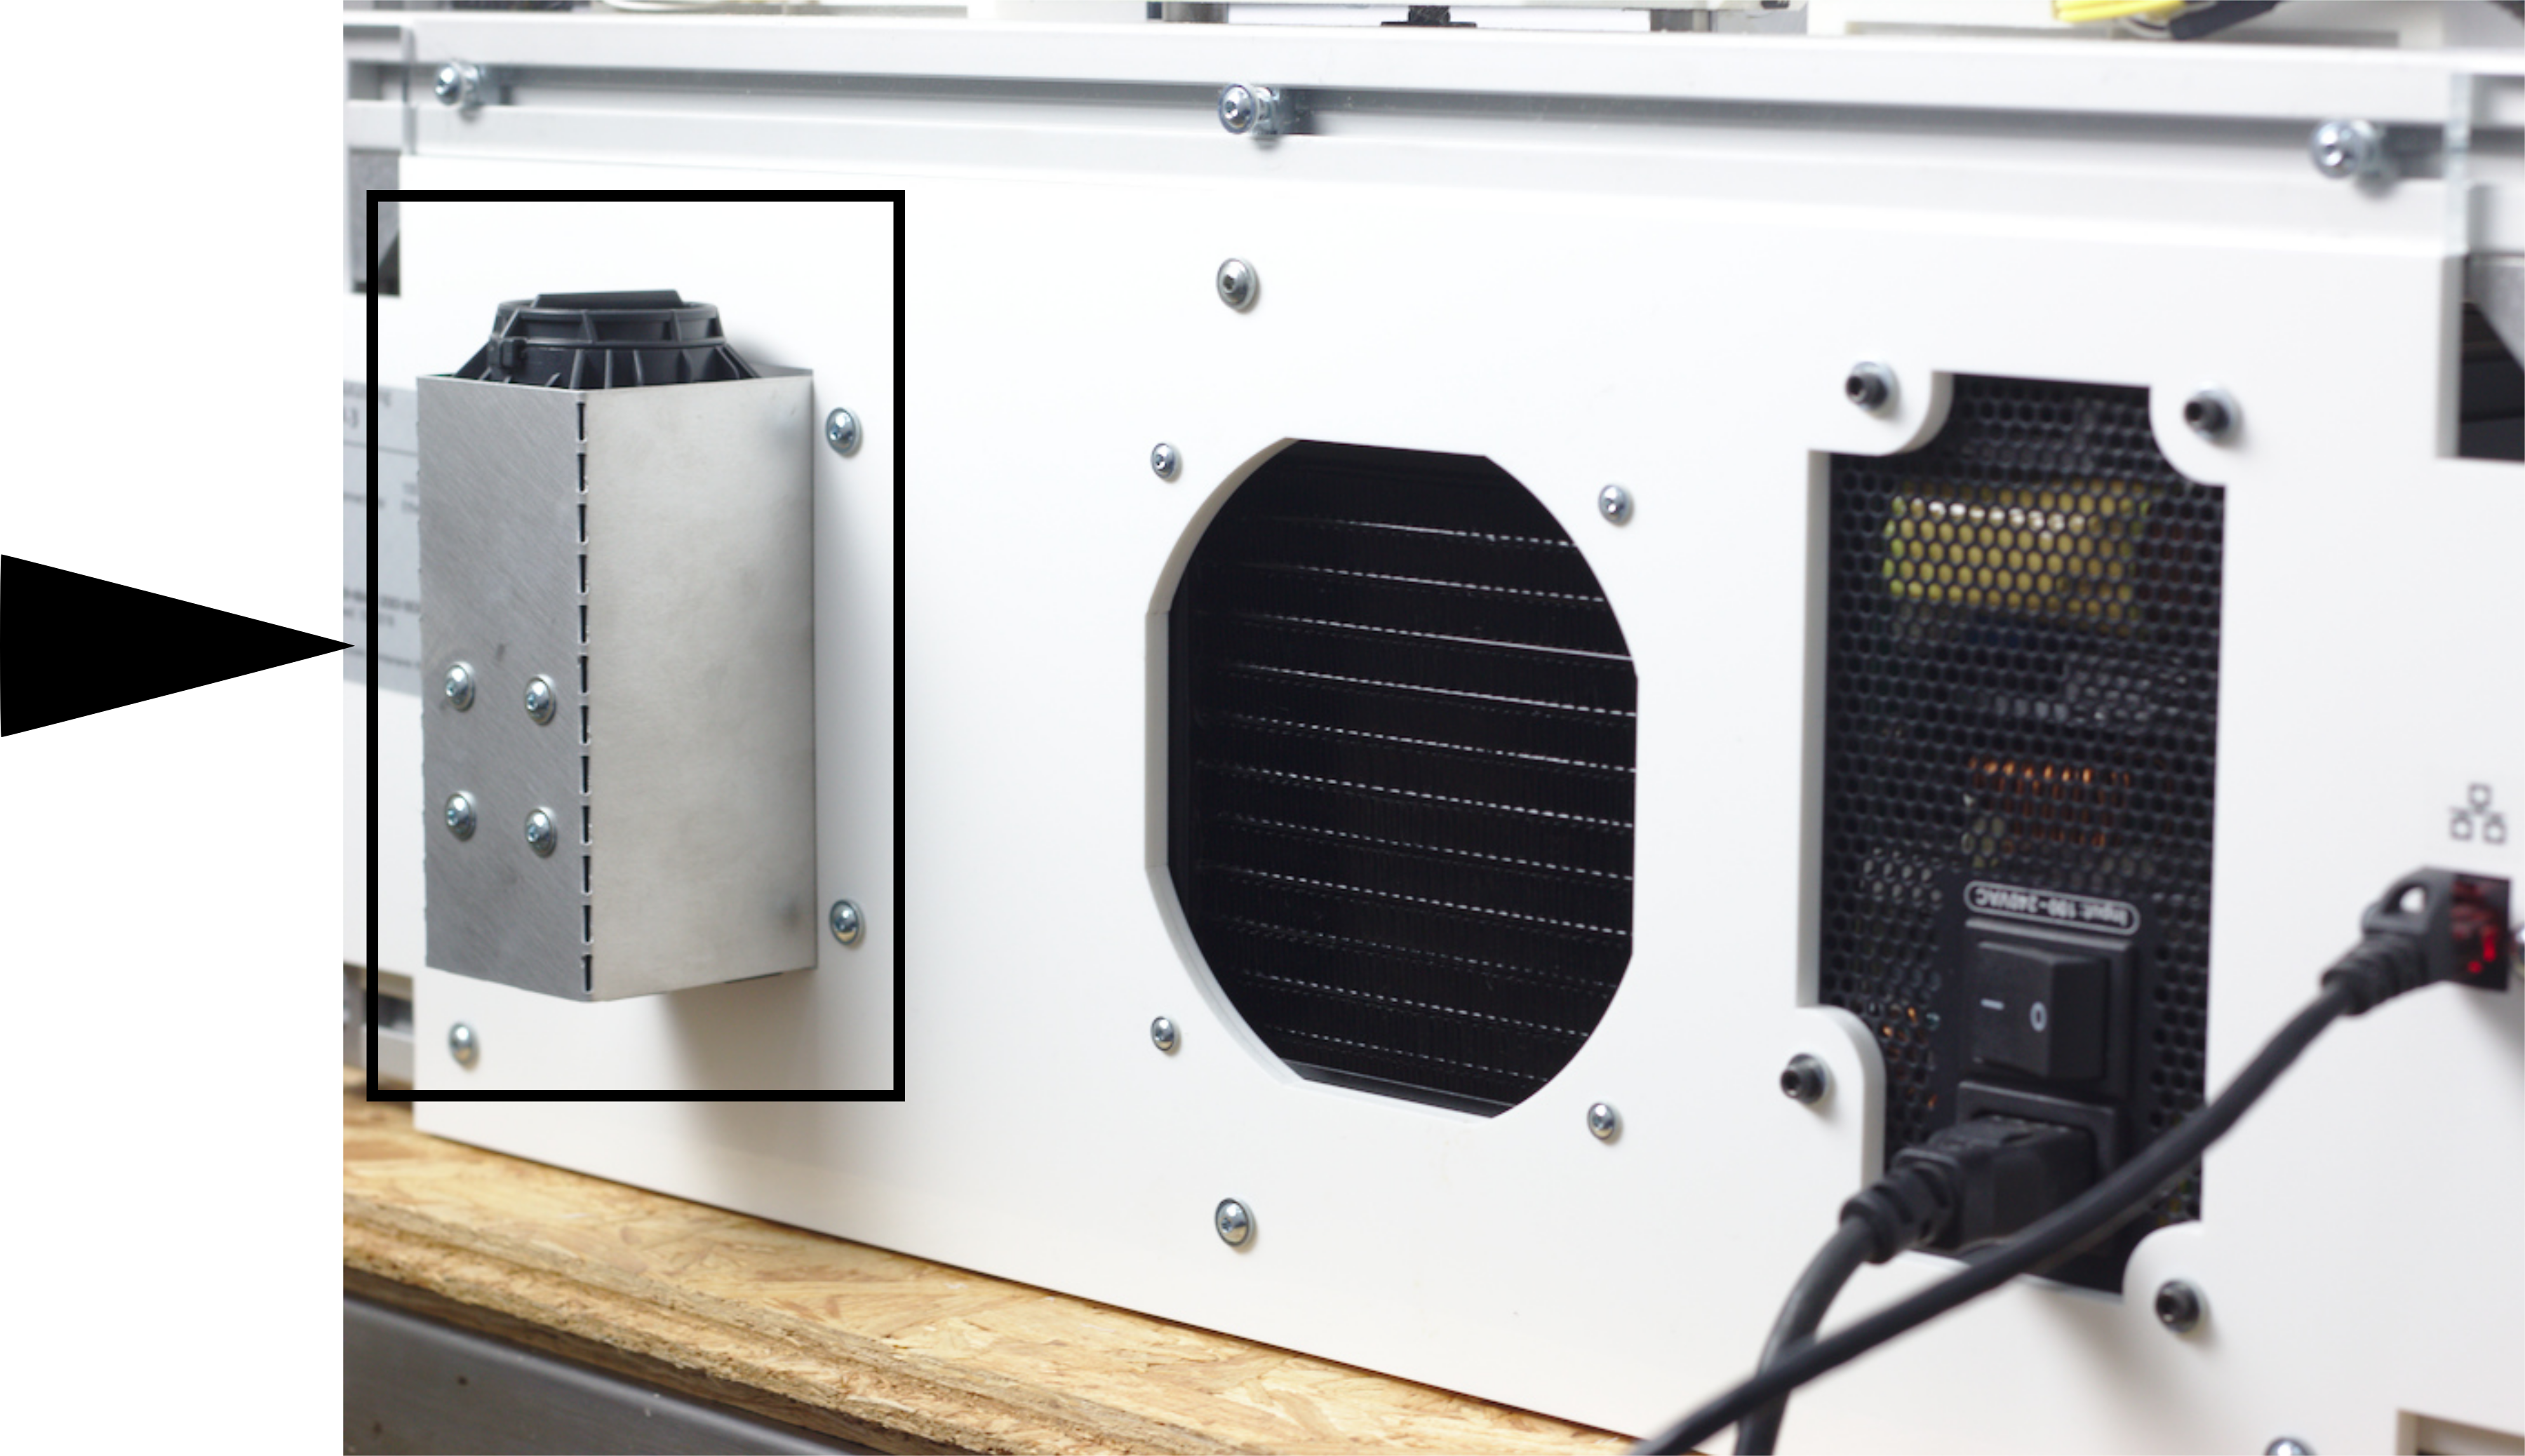
\includegraphics[width=.7\linewidth]{./img/waterpump_rear.png}
  \caption{Cooling water pump accessible at the rear of the machine.}    
\end{figure}

\begin{figure}[H]
  \centering
  \includegraphics[width=.7\linewidth]{./img/mtc_coolingwaterpumpopenlid.png}
  \caption{Opening/closing the pump's lid.}
\end{figure}

\begin{figure}[H]
  \centering
  \includegraphics[width=.7\linewidth]{./img/mtc_coolingwaterpumprefill.png}
  \caption{Level indication of the cooling water pump.}
\end{figure}


\subsubsection{Extruder idler lever}

\paragraph{Required tools}

\begin{itemize}
  \item Allen wrench \#3 
\end{itemize}	

\paragraph{Adjusting the preload}

At delivery, the idler lever preload is preset to work with the standard material \emph{Kühling\&Kühling ABS}. To print other plastics it may be necessary to adjust or readjust the tension of the idler lever spring. 

\begin{info}
  The preset value can be read as the distance in mm between the underside of the set screw and the underside of the extruder head carrier. It is set to 5.4 mm at delivery for ABS.
  \begin{figure}[H]
    \centering
    \includegraphics[width=.7\linewidth]{./img/mtc_idlerleverpreset.png}
  \end{figure}
\end{info}

Too high tension of the idler lever spring may result in the gear drive to slip and grind into the filament. Too low tension of the idler lever spring may result in slipping of the gear drive. In both cases the print will abort due to insufficient material transport.
Adjust the idler lever spring pressure by turning the tensioning screw with a metric \#3 Allen key, just enough that the filament is transported reliably without slipping or chipping. Turn the screw clockwise to increase the preload and counterclockwise to decrease it.
To test material transport efficiency run the Prime Extruders wizard and readjust if necessary. 

\begin{figure}[H]
  \centering
  \includegraphics[width=.7\linewidth]{./img/mtc_springload.png}
  \caption{Adjusting the idler lever preload.}
\end{figure}

\begin{info}
  Be gentle, too much pressure is counterproductive and will result in chipping filament.
\end{info}

\subsubsection{Timing Belt Tension} \label{sec:belttension}

The Tension of the X-axis and both Y-axis timing belts can be checked by measuring the resonance frequency when plucked like a guitar string.

\begin{itemize}
  \item Activate the build chamber preheating and wait until the 3D Printer 
        has reached its operating temperature (eg. 70\degree C for printing ABS).
  \item Then pluck the longest free hanging section of a belt and measure the oscillation with a frequency meter.
        Make sure to be as close to the belt as possible with the microphone of your device.
  \item Adjust by rotating the knurled thumb-wheels on each belt tensioner 
        until a frequency of about 60 Hz ($\pm$ 5 Hz) is met.
  \item Repeat this procedure for all belts.
\end{itemize}

\begin{figure}[H]
  \centering
  \includegraphics[width=.7\linewidth]{./img/mtc_belttension.png}
  \caption{Knurled thumb-wheels on belt tension}
\end{figure}

\begin{info}
  A guitar tuning device will be sufficient - also available as smart phone app.
\end{info}


\subsubsection{Repositioning and refastening the Z-axis clamp collar} \label{sec_spindlecollar}

During transport or set up verberation may lead to loosening of set screws. If this happens at the upper clamp collar of the Z-spindle, the initial Z-positioning of a print job becomes inaccurate \emph{although the leveling seems OK} because the spindle's mechanical backlash will then avert exact positioning only during minimal lifting moves. You will find that the first layer will not stick to the print bed as if it was leveled too high.
In this case the clamp collar must be repositioned and the set screw must be refastened. 

\paragraph{Required tools}

\begin{itemize}
  \item Allen key \#2.5
\end{itemize}

\paragraph{Testing and repositioning the clamp collars}

\begin{danger}
  OF BURNING\\
  Depending on the printed material components of the 3D Printer may hold 
  temperatures up to 500\degree C (932\degree F) immediately after a print job.
  To avoid burning injuries:

  \begin{itemize}
    \item Switch off the preheating and wait until the 3D Printer 
          has cooled down to approximately 50\degree C (122\degree F).
    \item Check the current temperature at the display.
  \end{itemize}
\end{danger}

\begin{info}
  Lifting the print table at the front end may damage the Z-elevator assembly and the spindle. Also, leverage effects might effect a false impression of alleged play.
  Grab the print table at the Z-elevator near the bearings when trying to lift it.
  Make sure that you do not damage the Z-limit switch. 

  \begin{figure}[H]
    \centering
    \includegraphics[width=.7\linewidth]{./img/mtc_liftelevatorincorrect.png}
  \end{figure}
\end{info}

To test if the clamp collar has come loose, carefully try to lift the print table and observe the Z-drive pulley.
If the pulleys moves up and down, the clamp collar must be repositioned and the set screws refastened. 

\begin{figure}[H]
  \centering
  \includegraphics[width=.7\linewidth]{./img/mtc_liftelevatorwatchpulley.png}
  \caption{Try to lift the Z-elevator and watch the pulley. If the pulley moves up and down, 
           the clamp collar must be repositioned.}
\end{figure}

To reposition the clamp collar:

\begin{itemize}
  \item Carefully turn the spindle of the Z-drive manually so that the recess of the clamp collar points left.
    
    \begin{figure}[H]
      \centering
      \includegraphics[width=.7\linewidth]{./img/mtc_z-axis_alignclampcollar.png}
      \caption{Align the recess of the clamp collar parallel to the 3D Printer's front.}
    \end{figure}

  \item Loosen the set screw through the access bore in the carriage.

    \begin{figure}[H]
      \centering
      \includegraphics[width=.7\linewidth]{./img/mtc_z-axis_loosensetscrew.png}
      \caption{Use the \#2 Allen key to loosen the set}
    \end{figure}

  \item Hold down the Z-pulley and push the clamp collar up to the limit.
  \item Hold the clamp collar in place and fasten the set screw tightly.

    \begin{figure}[H]
      \centering
      \includegraphics[width=.7\linewidth]{./img/mtc_z-axis_pushclampcollarup.png}
      \caption{Hold down the pulley and push up the clamp collar.}
    \end{figure}
\end{itemize}



\subsection{Electronic components, software and slicing}

\subsubsection{Exchanging the operating system SD card}

In case an update of the operating system, the touchscreen interface or the firmware is required, \emph{Kühling\&Kühling} offer update files at http://docs.kuehlingkuehling.de/. 

The Micro-SD card in the UDOO always contains all data necessary to run the operating system as a stand-alone unit, which means that you do not have to overwrite the current operating system but can use a second SD card to replace the original one. 

\paragraph{Updating procedure}

\begin{itemize}
  \item Finish all print jobs and turn the operating system off 
        via the touchscreen (\lbrack Shut-down\rbrack  button).
  \item Let the 3D Printer cool down.
  \item Toggle the main switch at the back off the apparatus to \emph{<0>} (OFF) and 
        remove the power supply cable.
  \item Remove the left side cover of the electronics enclosure (removal procedure as described here).
  \item Carefully remove the SD card deeper from its slot at the lower edge of the UDOO board. 
        The card is positioned behind the heatsink and has a \dq push and release\dq removal mechanism.
  \item Insert the new SD card into the slot.
  \item Reinstall the side cover of the electronic enclosure.
  \item Plug in the power supply cable.
  \item Switch the 3D Printer on by toggling the main switch to \emph{<I>} (ON).
\end{itemize}

\begin{figure}[H]
  \centering
  \includegraphics[width=.7\linewidth]{./img/sg_sd-card_removal.png}
  \caption{SD card slot at the lower edge of the UDOO board behind the heatsink.}
\end{figure}

After the start-up sequence has finished, the HT500.3 is now running with the updated operating system. 
